\subsubsection{PS58F1}

El módulo \texttt{PS58F1} es un controlador de tensión con un relé que se puede utilizar para muchas aplicaciones. En nuestro caso, nos interesaba la aplicación como controlador de descarga para la batería de plomo ácido, de manera que desconectara la batería cuando esta sobrepasara un umbral.

\begin{figure}[H]
    \centering
    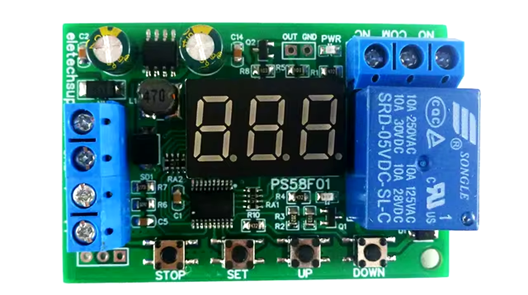
\includegraphics[width=0.5\textwidth]{images/2-hardware/componentes/PS58F1.png}
    \caption{Controlador de descarga \texttt{PS58F1}}
    \label{fig:hardware/modulos/controlador_descarga}
\end{figure}

Este módulo cuenta con un relé que es el que se utiliza para la conexión o desconexión de la batería. Sin embargo, este módulo cuenta con muy poca documentación. Además, tras conseguir configurarlo para que aproximadamente funcione, hemos apreciado que cuenta con una muy baja precisión y la utilización de un relé hace que cuente con un consumo no despreciable. Como punto final, la conmutación es inestable y a veces oscila en lugar de realizar una desconexión permanente.

Por todos estos factores, hemos decidido desechar este módulo y realizar un control de la descarga por software. Este control se explicará más profundamente en \todo{Enlazar a parte de control de descarga}. 